\begin{figure*}
\centering
\begin{tabular}{lc}
    \rotatebox[origin=l]{90}{\bf \;\,\quad\quad\quad\quad\quad\quad$k$-Median} &
    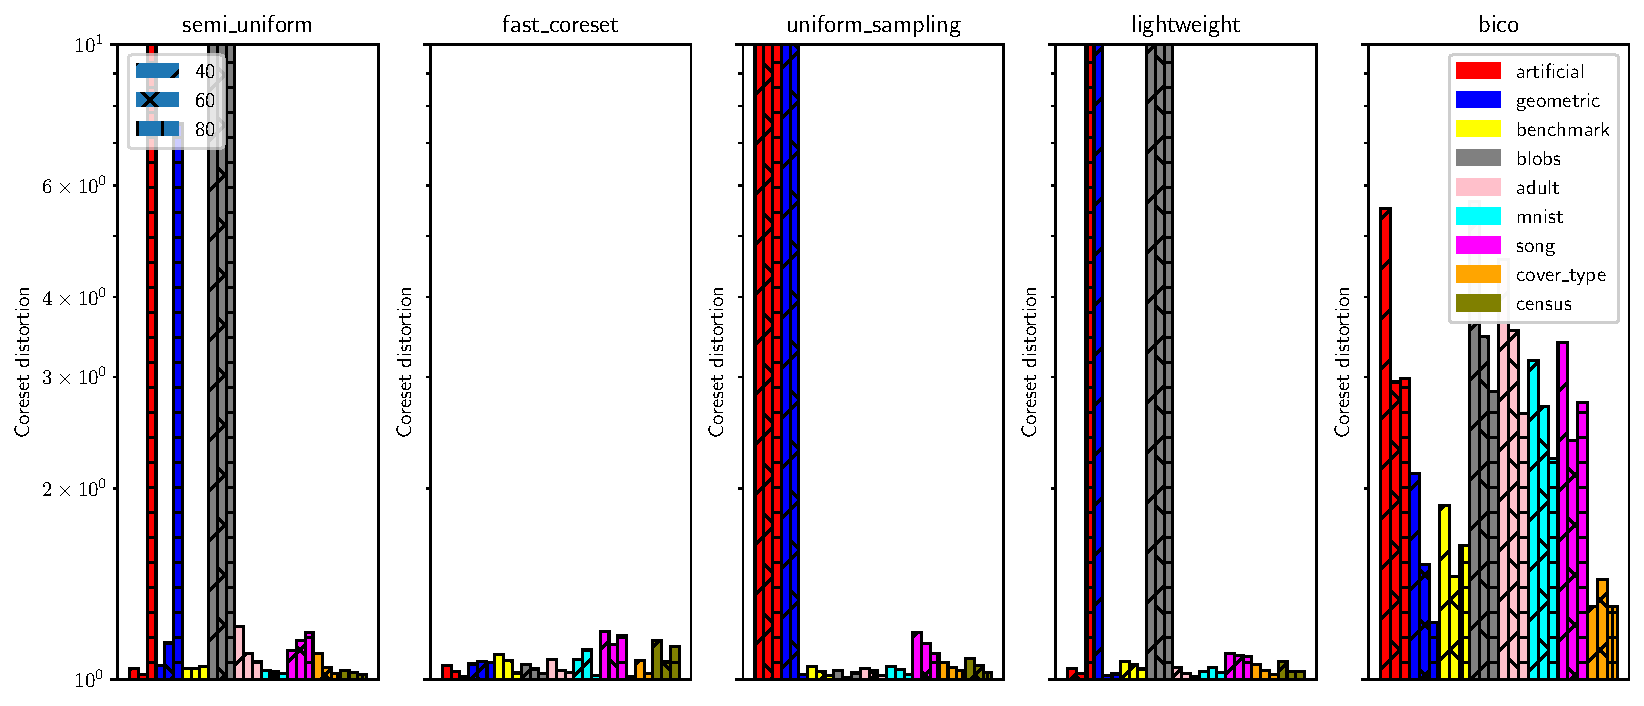
\includegraphics[width=.95\linewidth]{images/1/coreset_distortion-m_scalar_across_all_algorithms.pdf} \\

    \rotatebox[origin=l]{90}{\bf \;\;\quad\quad\quad\quad\quad\quad$k$-Means} &
    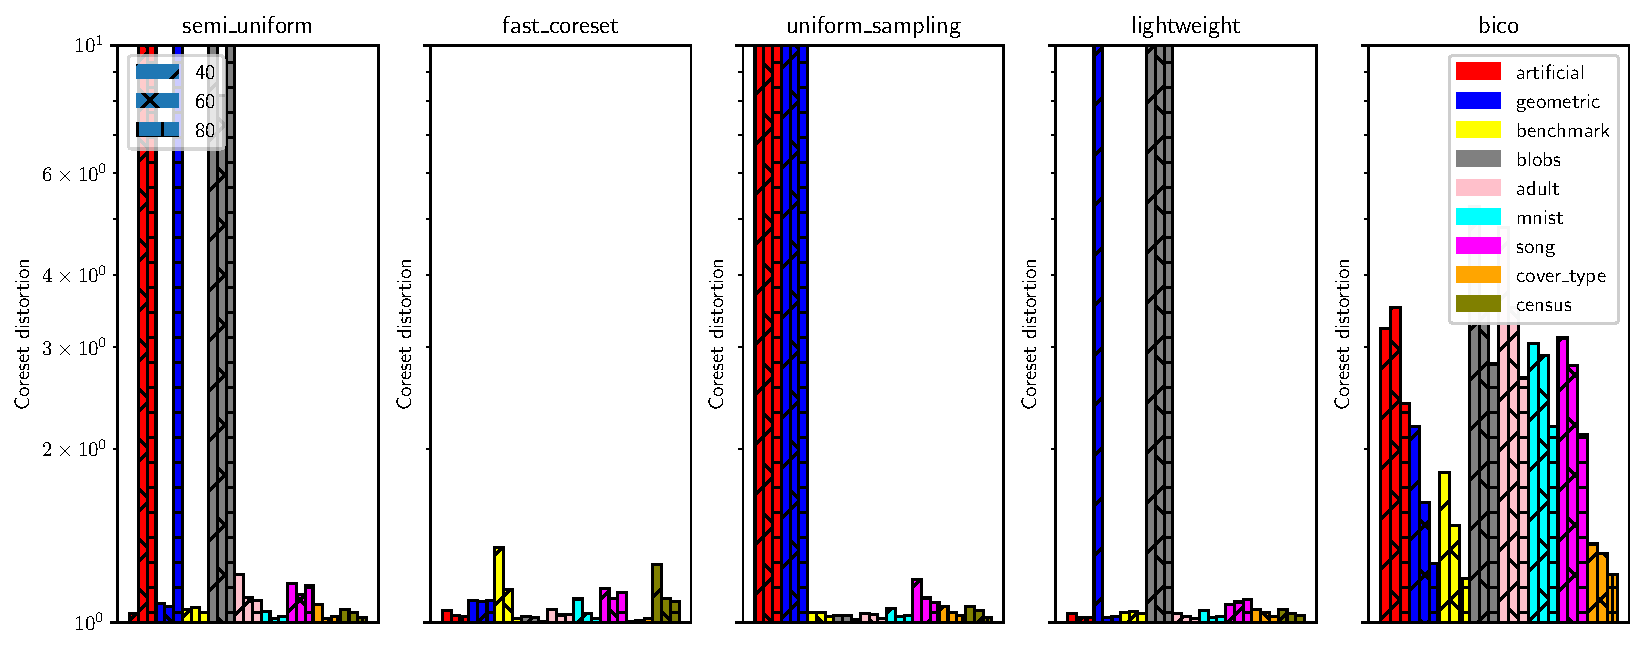
\includegraphics[width=.95\linewidth]{images/2/coreset_distortion-m_scalar_across_all_algorithms.pdf} \\

    \rotatebox[origin=l]{90}{\bf \;\quad\quad\quad\quad\quad\quad$k$-Means} &
    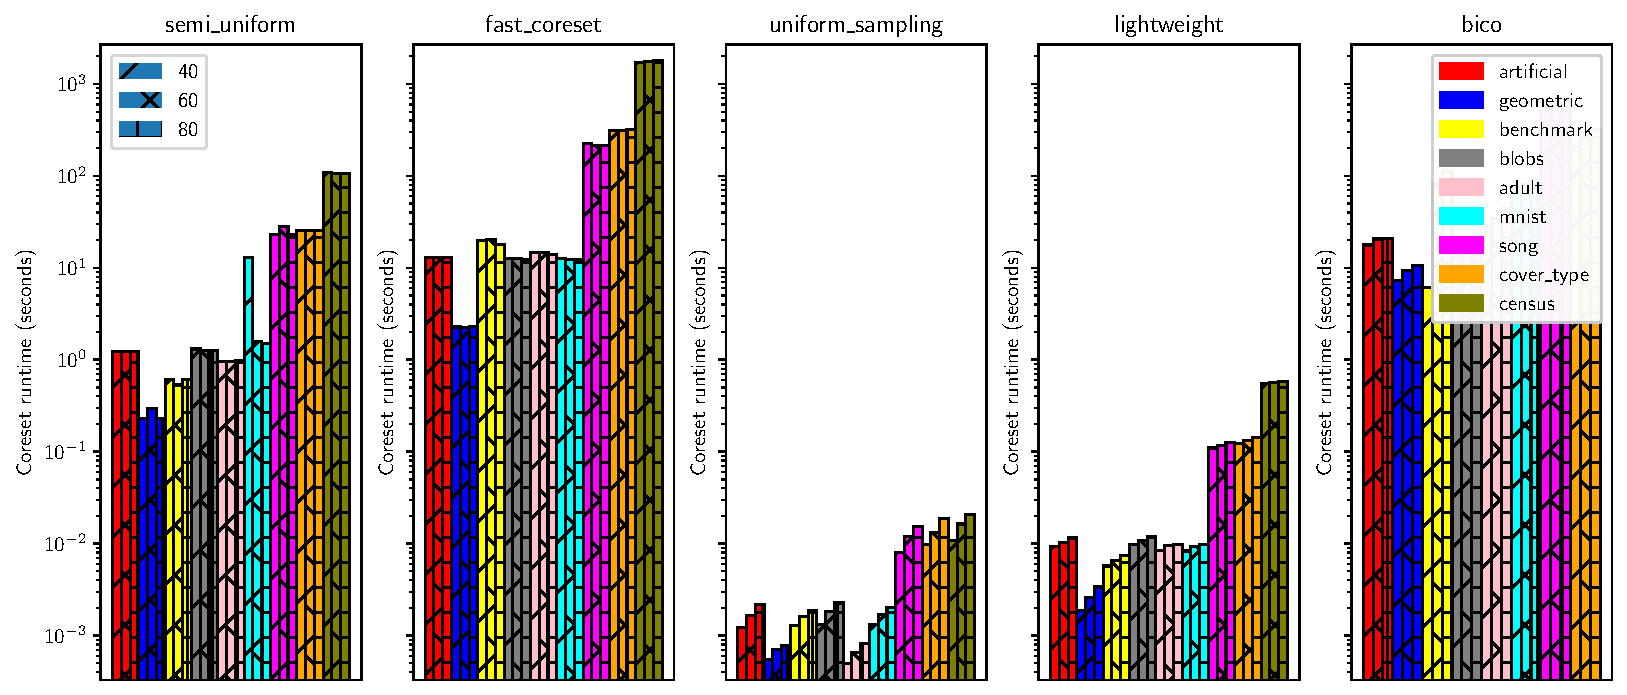
\includegraphics[width=.95\linewidth]{images/2/coreset_runtime-m_scalar_across_all_algorithms.pdf}
\end{tabular}
\caption{\emph{Top}: The effect of the $m$-scalar on the distortion metric for $k$-median.
\emph{Middle}: The effect of the $m$-scalar on the distortion metric for $k$-means.
\emph{Bottom}: The effect of the $m$-scalar on the algorithm runtime for $k$-means.
Notice that sensitivity sampling is the only fast method that consistently finds low-distortion coresets across the datasets.}
\label{fig:coreset_size_on_quality}
\end{figure*}
